\documentclass{article}
\usepackage[margin=1cm]{geometry}
\usepackage{tikz}

\begin{document}

\pagestyle{empty}

\begin{center}
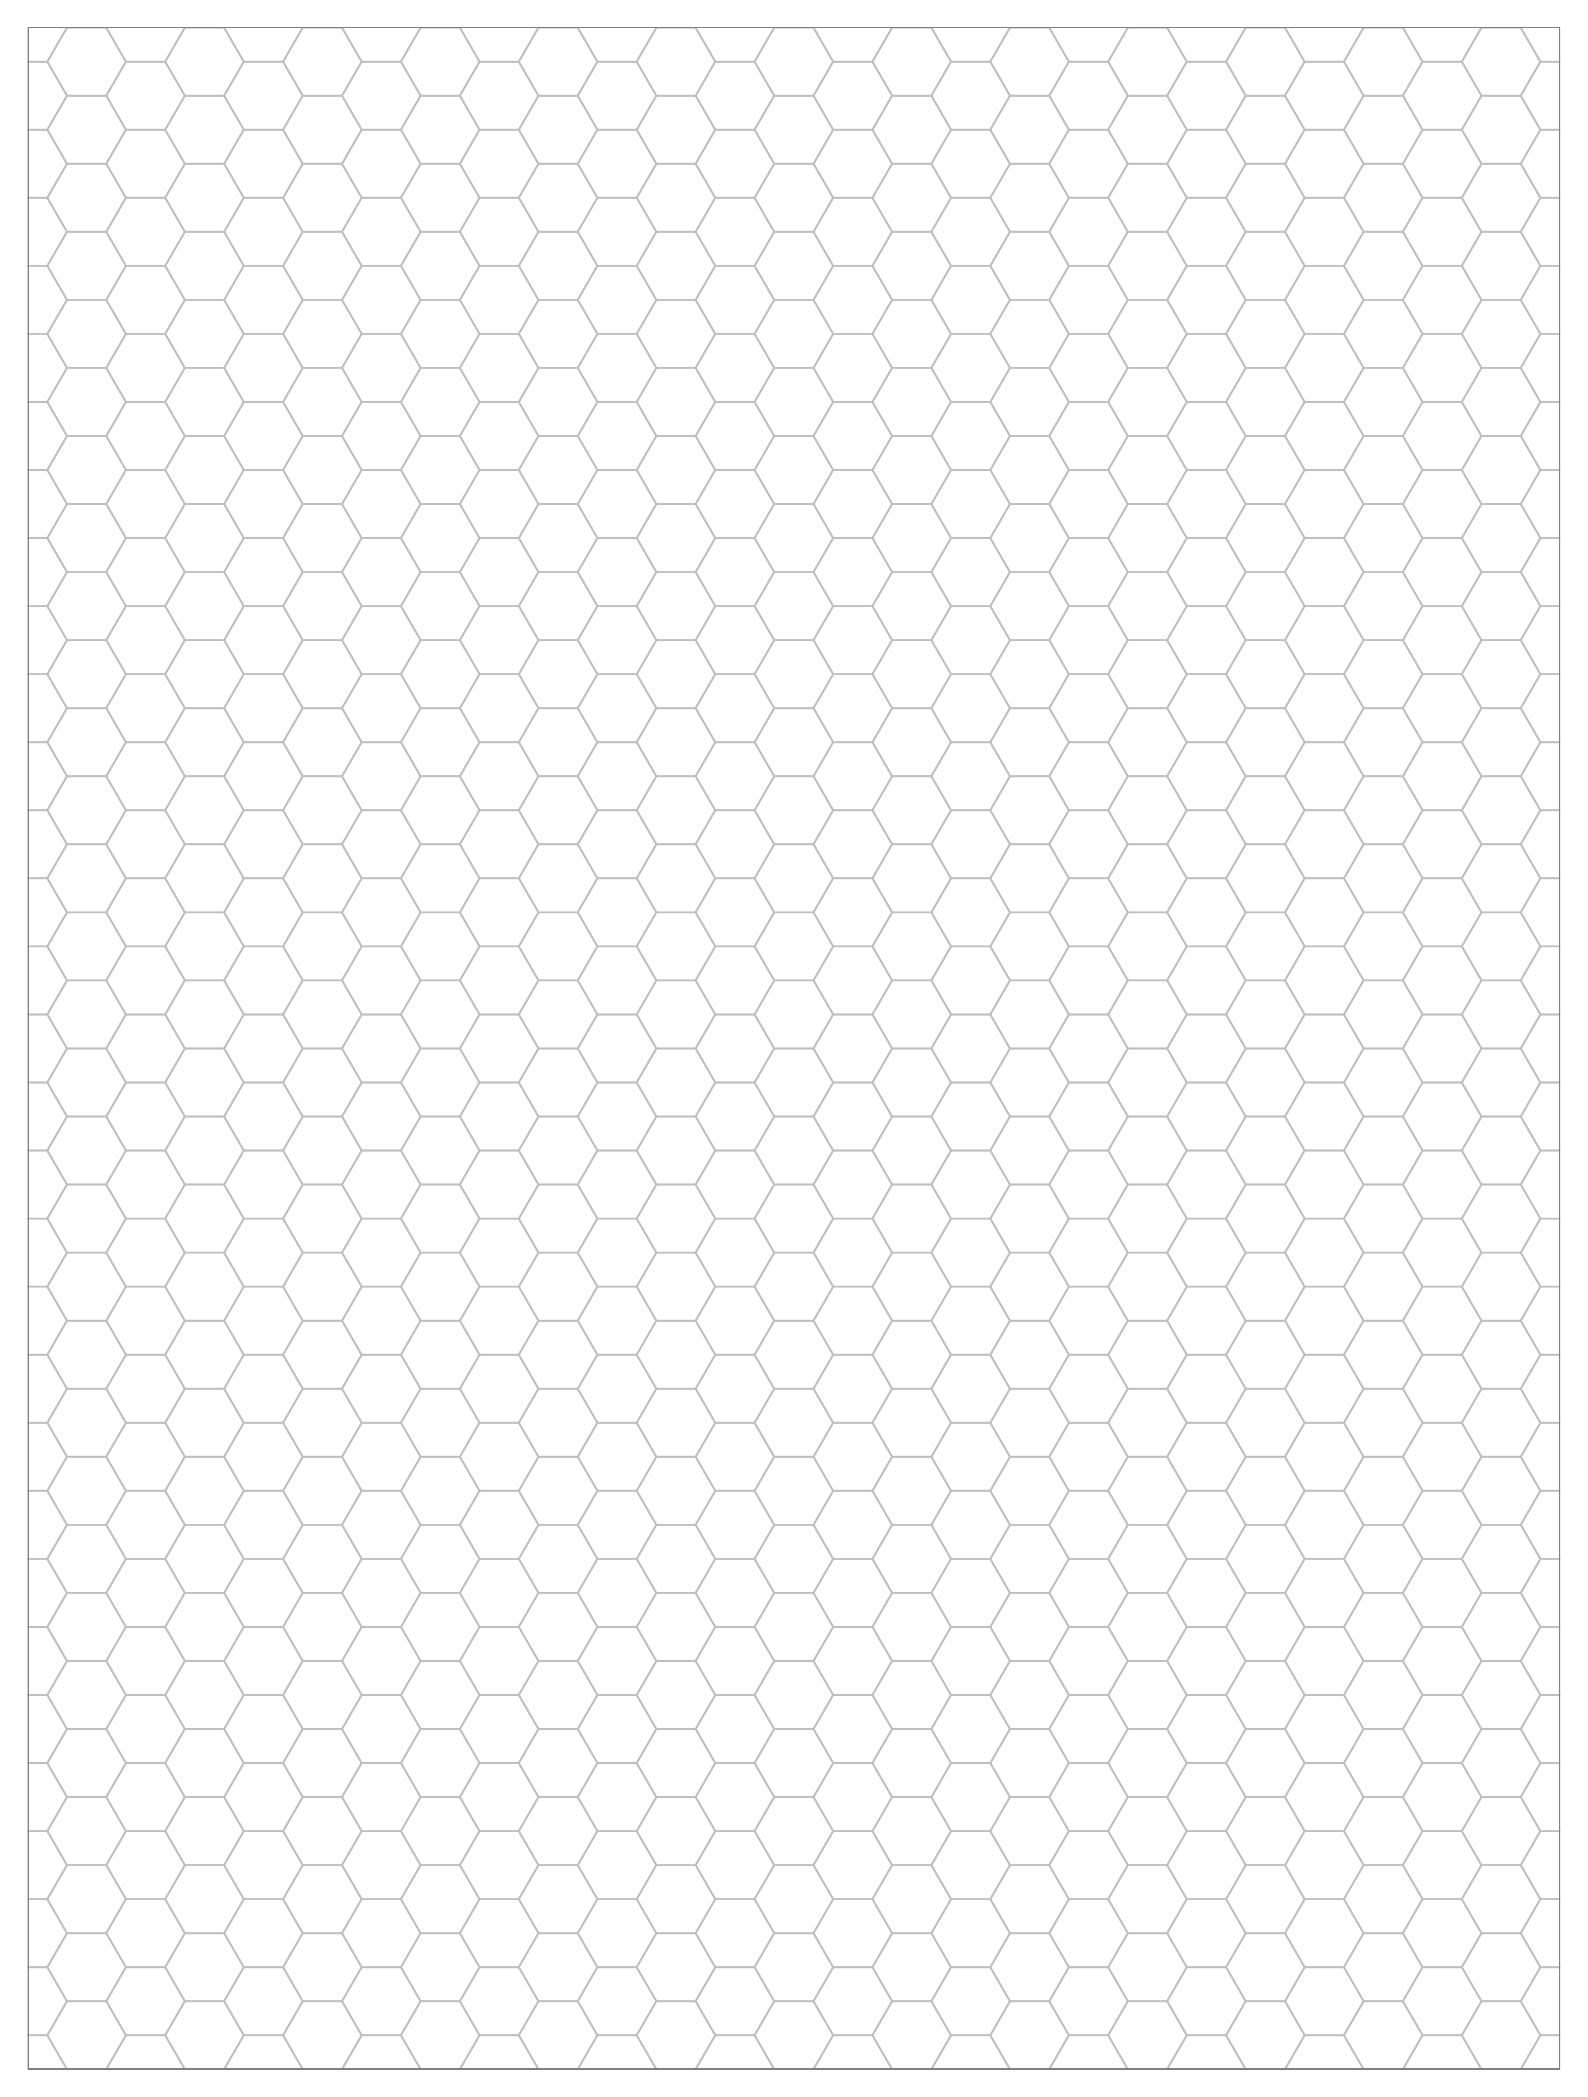
\begin{tikzpicture}[scale=0.499, yscale=1, xscale=1, rotate=0]
  \pgfmathsetmacro{\h}{31-1}
  \pgfmathsetmacro{\w}{14-1}

  \clip (0,0) rectangle (3*\w, {sqrt(3)*\h});

  \foreach \x in {0,...,\h} {%
    \foreach \y in {0,...,\w} {%
      \draw [line width=0.6, color=lightgray]%
        (3*\y,{sqrt(3)*\x})++(0:1) -- ++(120:1)%
          -- ++(180:1) -- ++(240:1) -- ++(300:1)%
          -- ++(360:1) -- ++(60:1);%
      \draw [line width=0.6, color=lightgray]%
        (1.5+3*\y,{sqrt(3)*(0.5+\x)})++(0:1)%
          -- ++(120:1) -- ++(180:1) -- ++(240:1)%
          -- ++(300:1) -- ++(360:1) -- ++(60:1);%
    }%
  }%

  \draw [color=gray, line width=0.6] (0,0) rectangle (3*\w, {sqrt(3)*\h});
\end{tikzpicture}
\end{center}

\end{document}
